\documentclass[]{report}

\voffset=-1.5cm
\oddsidemargin=0.0cm
\textwidth = 480pt

\usepackage{framed}
\usepackage{subfiles}
\usepackage{graphics}
\usepackage{newlfont}
\usepackage{eurosym}
\usepackage{amsmath,amsthm,amsfonts}
\usepackage{amsmath}
\usepackage{color}
\usepackage{amssymb}
\usepackage{multicol}
\usepackage[dvipsnames]{xcolor}
\usepackage{graphicx}
\begin{document}


\section*{Checking for Normality}

\begin{itemize}
	\item A normal distribution is often a reasonable model for continuous data. However, without inspecting the data, it is risky to assume a normal distribution. \item  There are a number of graphical methods, for example histogram and boxplots, that can be used to indicate deviations of the data from the normal distribution. 
	
%	\item  A histogram is an example of a graph that can be used to check normality. Here, the histogram should reveal a bell shaped curve. 
\end{itemize}

\begin{figure}[h!]
	\centering
	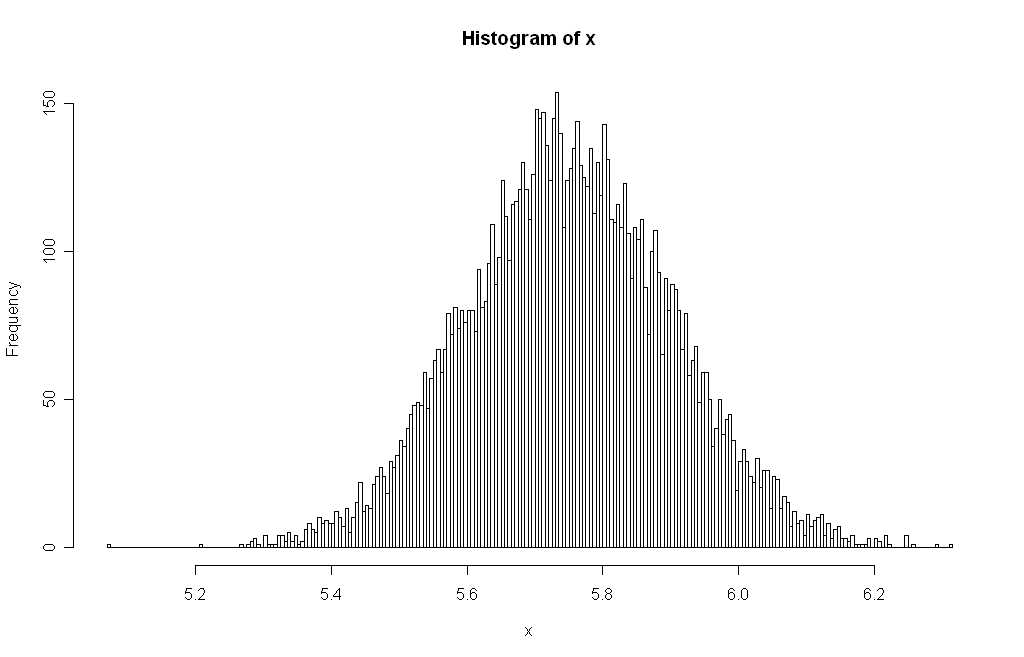
\includegraphics[width=0.55\linewidth]{images/normal}
\end{figure}



\subsection*{Normal Probability Plots (a.k.a Q-Q Plots)}

\begin{itemize}
	\item The most useful tool for assessing normality is a quantile quantile or QQ plot. This is a scatterplot with the quantiles of the scores on the horizontal axis and the expected normal scores on the vertical axis. 
	
	\item  The steps in constructing a QQ plot are as follows: 
	
	\begin{itemize}
		\item  The data is sorted from smallest to largest. A plot of these scores against the expected normal scores should reveal a straight line. \item The expected normal scores are calculated by taking the z-scores  where I is the rank in increasing order.
	\end{itemize}
	
	\item  Curvature of the points indicates departures of normality. \item  This plot is also useful for detecting outliers. The outliers appear as points that are far away from the overall pattern op points
\end{itemize}




\subsection{Graphical Methods}

\begin{itemize}
	\item The quantile-quantile (QQ) plot is an excellent way to see whether the data deviate from normal (the plot can be set up to see if the data deviate from other distributions as well but here we are only interested in the normal distribution). The process SPSS goes through for creating a QQ plot involves determining what proportion of the 'observed' scores fall below any one score, then the z score that would fit that proportion if the data were normally distributed is calculated, and finally that z score that would cut off that proportion (the 'expected normal value') is translated back into the original metric to see what raw score that would be. 
	
	\item A scatter plot is then created that shows the relationship between the actual 'observed' values and what those values would be 'expected' to be if the data were normally distributed. 
	\item Interpretation is straightforward: if the data are normally distributed then the circles on the resulting plot (each circle representing a score) will form a straight line. 
	
	%Use the following examples to learn how to interpret QQ plots, be aware that some stat programs switch the axes around from the way it is set up in SPSS.
\end{itemize}





%-------------------------------------------------------------------------- %

\subsection{Normal Probability Plots}

\begin{itemize}
\item A histogram is an example of a graph that can be used to check normality. \item Here, the histogram should reveal a bell shaped curve. 
\end{itemize}
\begin{figure}
\centering
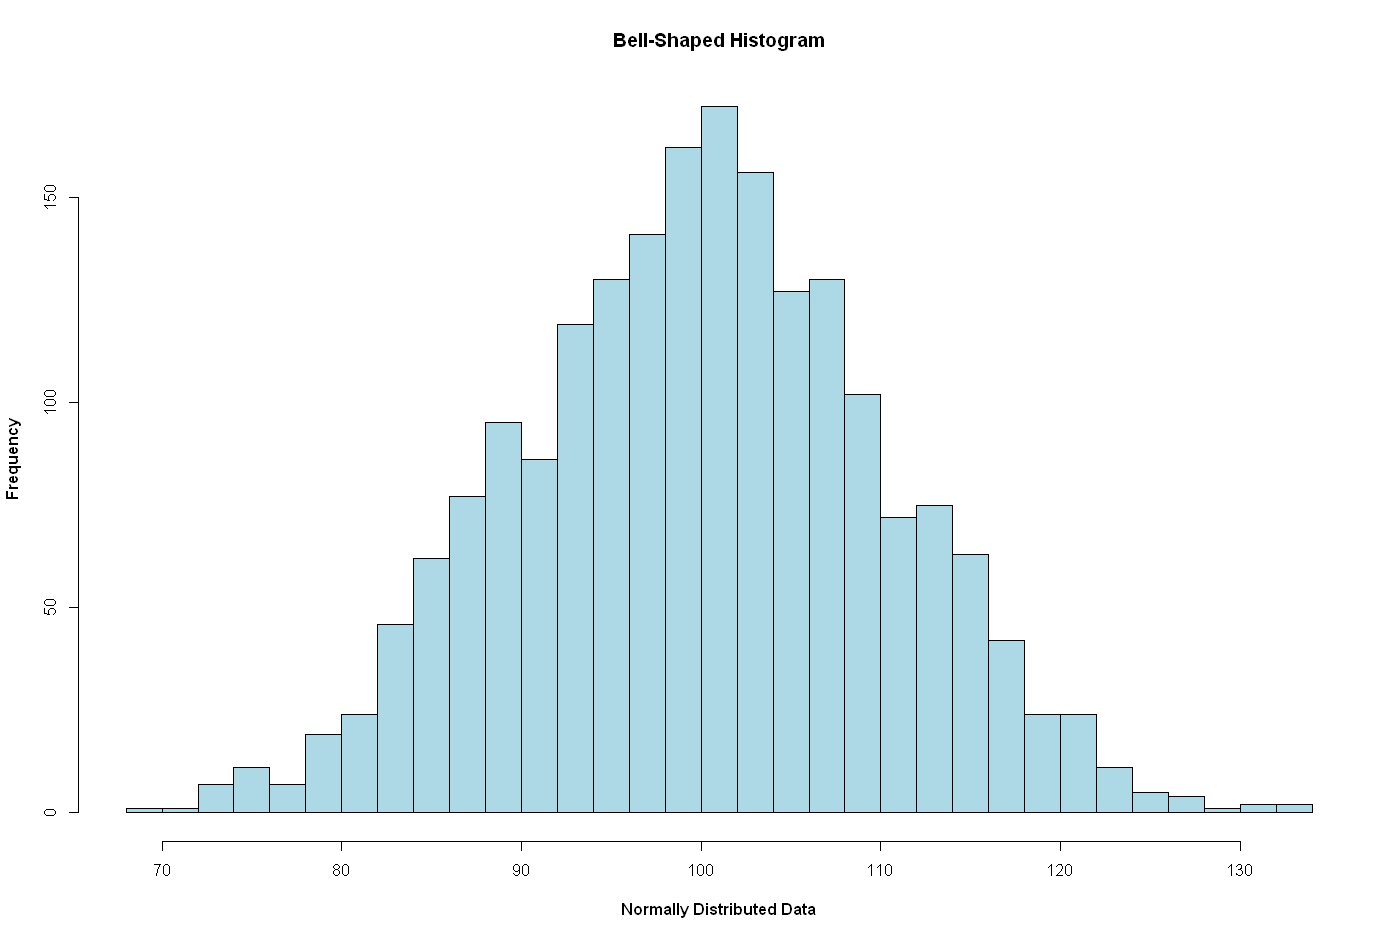
\includegraphics[width=0.7\linewidth]{images/LargeXNormHist}
\caption{}
\label{fig:largexnormhist}
\end{figure}



\begin{figure}
\centering
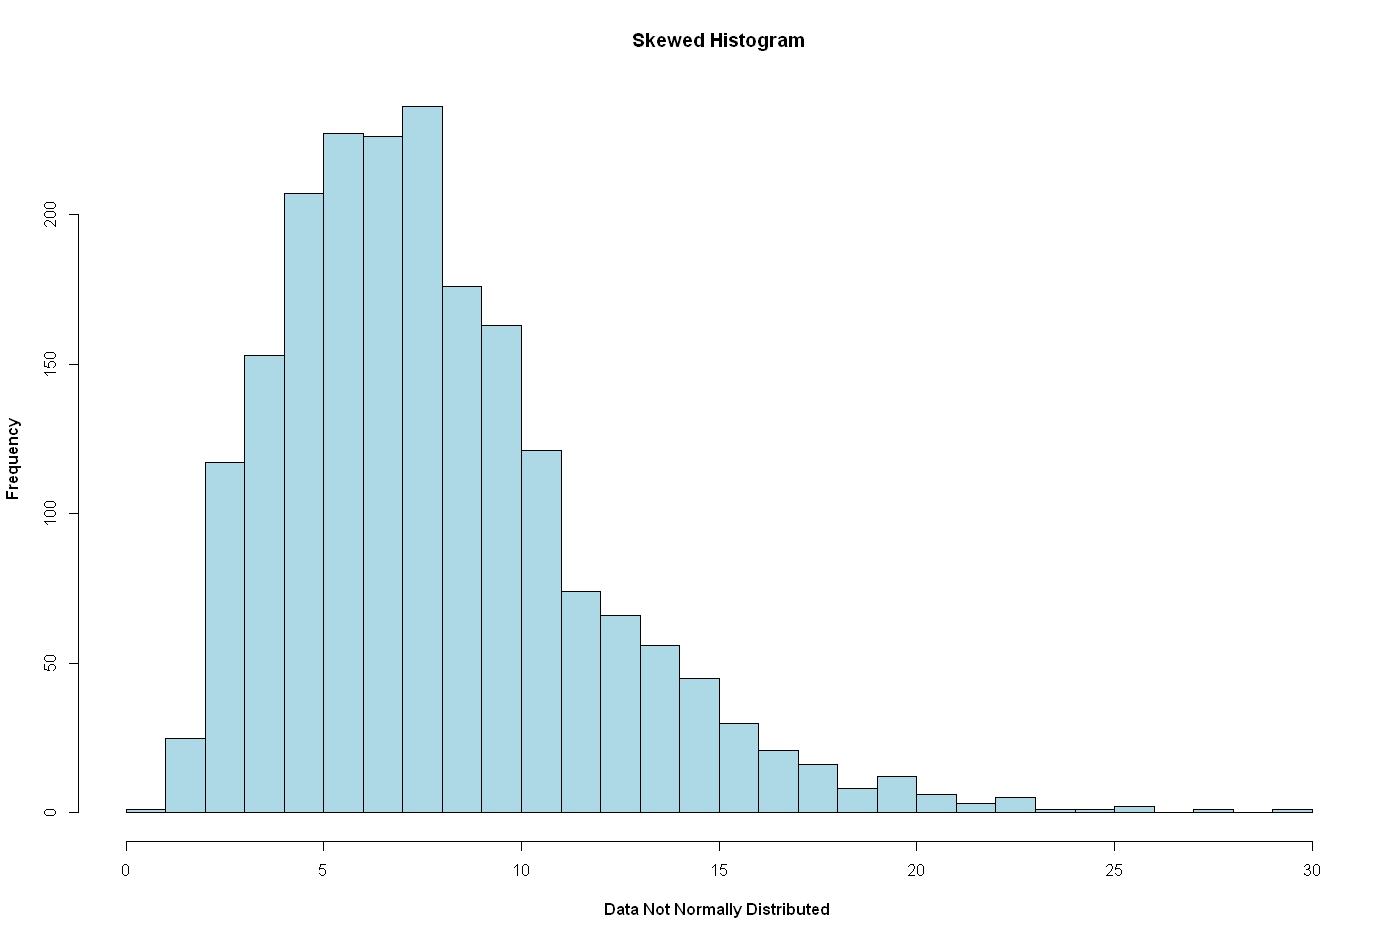
\includegraphics[width=0.7\linewidth]{images/LargeXNotNormHist}
\label{fig:LargeXNotNormHist}
\end{figure}


\begin{itemize}

\item The most useful tool for assessing normality is a \textit{\textbf{quantile -quantile}} or \textbf{Q-Q} plot. \item This is a scatterplot with the quantiles of the scores on the horizontal axis and the equivalent values expected when assuming the normal distribution, on the vertical axis. 
\end{itemize}


\begin{itemize}
\item The steps in constructing a QQ plot are as follows: First, we sort the data from smallest to largest. 
\item A plot of these scores against the expected normal scores should reveal a straight line. \item The expected normal scores are calculated by taking the z-scores  where I is the rank in increasing order.
\end{itemize}


\begin{itemize}

\item Curvature of the points indicates departures of normality. This plot is also useful for detecting outliers. The outliers appear as points that are far away from the overall pattern op points
\end{itemize}

\end{document}
